\section{Theoretischer Hintergrund}
In diesem Kapitel werden die theoretischen Grundlagen vorgestellt, die für das Ver\-ständ\-nis und die Umsetzung der in dieser Arbeit behandelten Konzepte notwendig sind.
Dazu gehören Methoden zur Beschreibung der Position und Orientierung eines Roboters sowie verschiedene mathematische Modelle für Rotationen.
Zudem wird der Differentialantrieb als typisches Fortbewegungsprinzip mobiler Roboter erläutert. Ergänzend wird das Softwarewerkzeug JupyterLab eingeführt,
das in dieser Arbeit zur interaktiven Entwicklung und Visualisierung verwendet wird.

\subsection{Darstellung der Position und Orientierung eines Roboters}
Ein Roboter wird in der Regel als ein unverformbarer fester Körper (Rigid Body) betrachtet, der sowohl eine bestimmte Position als auch eine Orientierung im Raum besitzt.
Die Position beschreibt den Abstand und die Verschiebung zwischen dem globalen Weltkoordinatensystem und dem körpereigenen Koordinatensystem des Roboters.
Die Orientierung hingegen gibt den Unterschied in der Winkelausrichtung zwischen dem Weltkoordinatensystem und dem lokalen Koordinatensystem des Roboters an.
Die Kombination aus Position und Orientierung eines Körpers wird als Pose bezeichnet. Die Transformation von einer Pose in eine andere kann intuitiv als Bewegung interpretiert werden.
Diese Transformation setzt sich aus einer Translation (Verschiebung) und einer Rotation (Drehung) zusammen \doublecite[24-27]{Robotics_Vision_and_Control}.
Speziell bei radgetriebenen Robotern wird die Pose auf einer Ebene beschrieben.
In diesem Fall besteht die Pose aus den X- und Y-Koordinaten im globalen Koordinatensystem sowie dem Winkel zwischen dem globalen und dem körpereigenen Koordinatensystem.
Damit lässt sich die Pose als ein Vektor aus diesen drei Elementen darstellen \doublecite[59]{autonomous_mobile_robots}.


\vspace{1em}

    \begin{figure}[H]
        \centering
        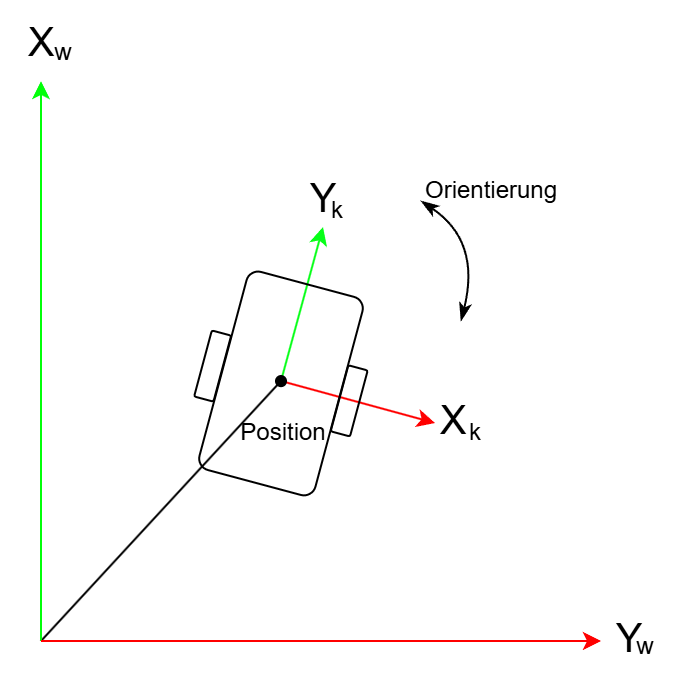
\includegraphics[width=0.7\textwidth]{images/position_orientierung.png}
        \caption{Ein Radgetriebender Roboter mit einem Körpereigenem Koordinatensystem in der X-Y-Ebene}
        \label{fig:Position_und_Orientierung}
    \end{figure}

\vspace{1em}


\subsection{Euler-Winkel und Roll-Pitch-Yaw-Winkel}
Euler’s Rotationstheorem besagt, dass zwei beliebige unabhängige,
orthonormale Koordinatensysteme durch eine Abfolge von maximal drei Rotationen um Koordinatenachsen miteinander in Beziehung gesetzt werden können,
wobei keine zwei aufeinanderfolgenden Rotationen um die gleiche Achse erfolgen dürfen \doublecite[136]{Quaternions_and_Rotation_Sequences_A_Primer_with_Applications_to_Orbits_Aerospace_and_Virtual_Reality}.
Das bedeutet, dass jede Rotation zwischen zwei Koordinatensystemen im dreidimensionalen Raum durch eine Sequenz von drei Rotationswinkeln beschrieben werden kann,
wobei jeder Winkel einer bestimmten Achse zugeordnet ist. Die Rotationen werden nacheinander ausgeführt:
Zunächst erfolgt eine Rotation des Weltkoordinatensystems um eine Achse, wodurch ein neues Koordinatensystem entsteht.
Anschließend wird dieses neue System um eine seiner eigenen Achsen rotiert, gefolgt von einer dritten Rotation um eine Achse des wiederum neu entstandenen Systems.
Dieser Vorgang wird in Abbildung~\ref{fig:Euler} illustriert.

\vspace{1em}

    \begin{figure}[H]
        \centering
        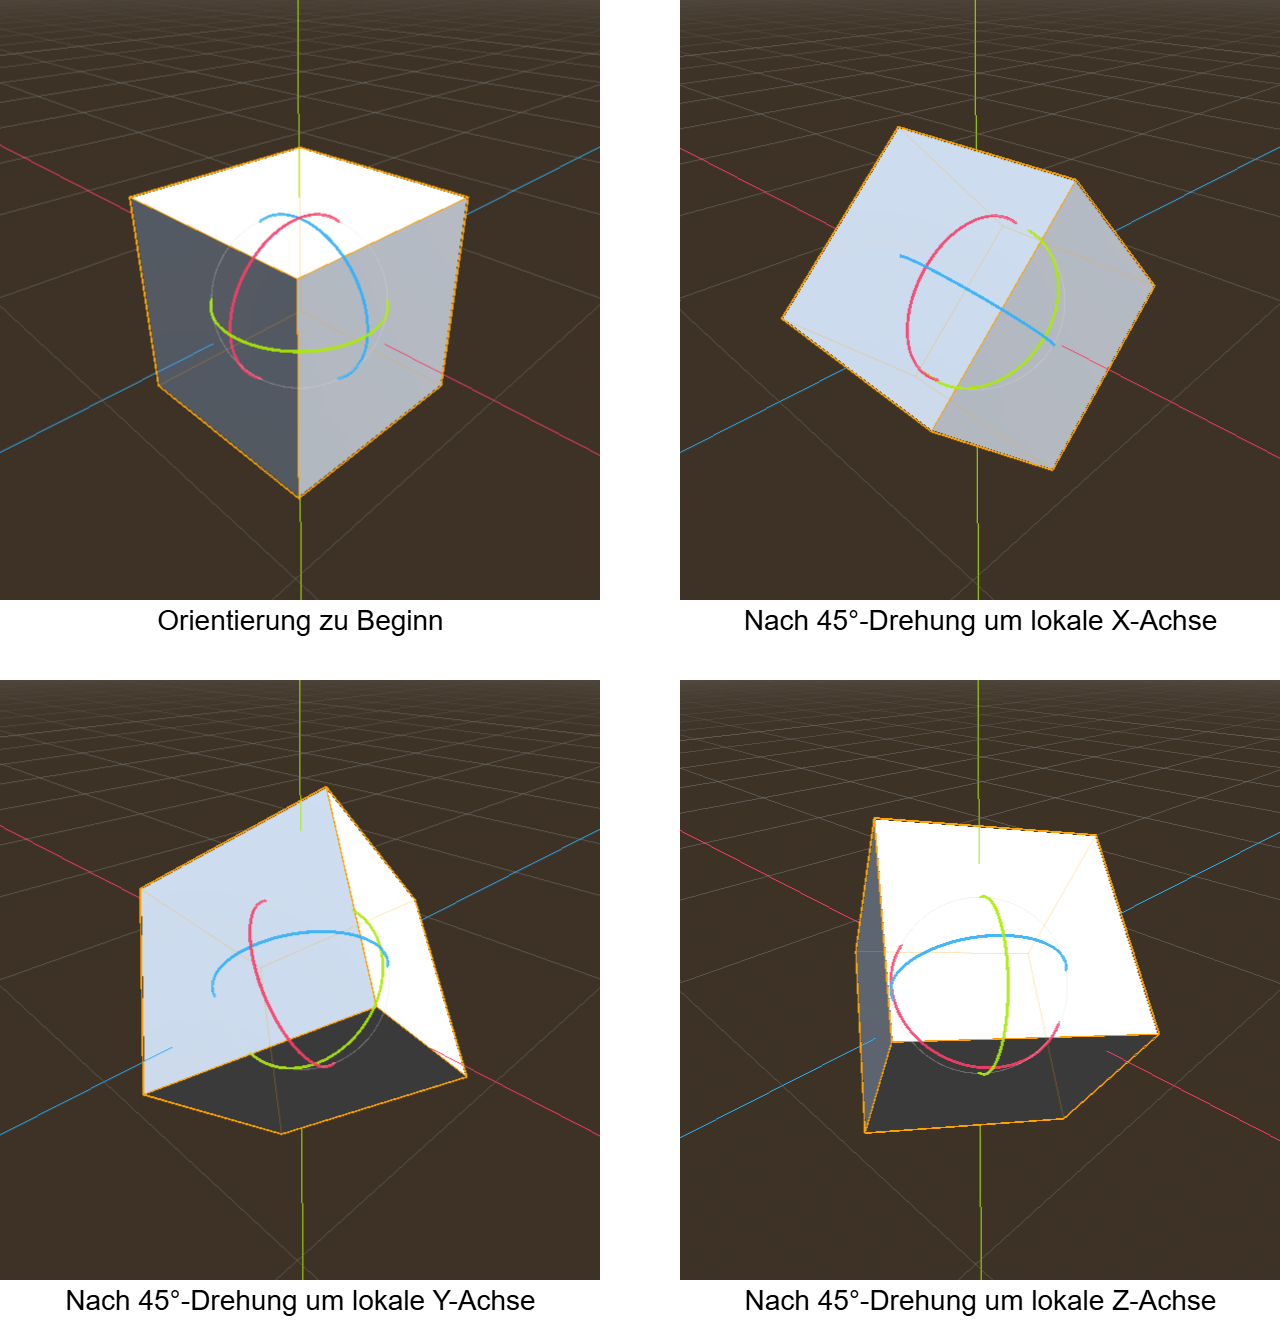
\includegraphics[width=0.7\textwidth]{images/euler.png}
        \caption{Eulerrotation eines Würfels um X, Y und Z in dieser Reihenfolge}
        \label{fig:Euler}
    \end{figure}

\vspace{1em}


In der Abbildung ist ein Würfel zu sehen, der durch drei aufeinanderfolgende Rotationen um sein jeweils aktuelles,
lokales Koordinatensystem gedreht wird. Zunächst erfolgt eine Rotation um 45° um die X-Achse.
Anschließend wird der Würfel um die daraus resultierende Y-Achse rotiert, gefolgt von einer letzten Drehung um die daraus entstehende Z-Achse.
Im Inneren des Würfels befindet sich ein sogenanntes Gimbal (kardanische Aufhängung), dessen Ringe anschaulich verdeutlichen,
in welcher Richtung die jeweilige Rotationsbewegung erfolgt.

Insgesamt gibt es zwölf eindeutige Rotationsabfolgen. Sechs davon beinhalten Wiederholungen derselben Achse (aber nicht unmittelbar hintereinander),
beispielsweise XYX, XZX, YXY, YZY, ZXZ oder ZYZ. Die anderen sechs Rotationsabfolgen verwenden jeweils alle drei Achsen einmal,
beispielsweise XYZ, XZY, YZX, YXZ, ZXY oder ZYX.

Der Begriff Euler-Winkel wird häufig verwendet, um jede Art von dreifacher Rotationsdarstellung zu bezeichnen.
Diese Bezeichnung ist jedoch nicht präzise, da je nach Reihenfolge der Rotationen verschiedene Darstellungen entstehen.
Deshalb muss die genaue Rotationsabfolge angegeben werden, auch wenn innerhalb bestimmter technischer Fachgebiete wie der Robotik meist die Konvention ZYZ herrscht.

Eine besondere Rolle spielen die sogenannten Roll-Pitch-Yaw-Winkel, bei denen es zwei gebräuchliche Rotationssequenzen gibt: ZYX und XYZ.
In der mobilen Robotik wird typischerweise die ZYX-Sequenz verwendet,
während bei stationären Robotermanipulatoren oft die XYZ-Sequenz Anwendung findet \doublecite[48-51]{Robotics_Vision_and_Control}.

\subsection{Rotationsmatrizen}
Eine Rotationsmatrix ist eine spezielle Art von Matrix, die ein Koordinatensystem um einen Winkel $\theta$ dreht und es dadurch in ein neues Koordinatensystem transformiert.
Die Spalten einer Rotationsmatrix können dabei als die transformierten Einheitsvektoren des ursprünglichen Koordinatensystems interpretiert werden.

Rotationsmatrizen sind stets orthonormal, das bedeutet, ihre Spalten (bzw. Zeilen) stehen senkrecht aufeinander und haben die Länge 1.
Daraus folgt die wichtige Eigenschaft:
\[
 R^{-1}=R^T
 \]
wobei $R^{-1}$ die Inverse und $R^T$ die Trasponierte der Matrix $R$ ist.
Ein weiteres charakteristisches Merkmal von Rotationsmatrizen ist, dass ihre Determinante stets den Wert $1$ hat.

Desweiteren sind sie Elemente der sogenannten speziellen orthogonalen Gruppe der Dimension 2, die als $SO(2)$ bezeichnet wird. Dies wird auch geschrieben als:
\[
    R \in \mathrm{SO}(2) \subset \mathbb{R}^{2 \times 2}
\]
Die spezielle orthogonale Gruppe ist eine Gruppe bezüglich der Matrixmultiplikation.
Das bedeutet, dass das Produkt zweier Rotationsmatrizen wieder eine Rotationsmatrix ist und somit ebenfalls zur Gruppe gehört.
Ebenso ist die Inverse jeder Rotationsmatrix ebenfalls Teil der Gruppe \doublecite[33]{Robotics_Vision_and_Control}.

\subsection{Quaternionen und Unit-Quaternionen}
Quaternionen wurden im Jahr 1843 von William Rowan Hamilton entdeckt. Sie erweitern die komplexen Zahlen und bestehen aus einem Skalar- und Vektoranteil:
 \[
 q=s+v_xi+v_yj+v_zk
 \]
 wobei $i$, $j$ und $k$ besondere Einheiten mit $i^2=j^2=k^2=ijk=-1$ sind.
 Der Skalaranteil ist eine einzelne reelle Zahl, während der Vektoranteil aus drei Komponenten besteht und einem dreidimensionalen Vektor entspricht.
 Quaternionen bilden einen Vektorraum: Man kann sie addieren, skalieren, multiplizieren (Hamilton-Produkt) und konjugieren. Die Multiplikation ist nicht kommutativ. Der Betrag eines Quaternions ist:
 \[
 ||q||=\sqrt{s^2+v_x^2+v_y^2+v_z^2}
 \]
 Unit-Quaternionen sind Quaternionen mit Betrag 1. Sie werden häufig verwendet, um Rotationen im Raum darzustellen. Eine Rotation um eine Achse $\hat{v}$ mit Winkel $\theta$ wird als
 \[
 q=\cos(\frac{\theta}{2})+\hat{v} \sin(\frac{\theta}{2})
 \]
bezeichnet. Quaternionen bieten bei der Darstellung von Rotationen mehrere Vorteile.
 Sie ermöglichen eine recheneffiziente Kombination von Rotationen und vermeiden dabei Probleme, wie den sogenannten Gimbal Lock,
 der bei der Verwendung von Euler-Winkeln auftreten kann.
 Dabei handelt es sich um den Verlust eines Freiheitsgrads,
 wenn zwei Rotationsachsen durch bestimmte Winkelkonstellationen aufeinander fallen und dadurch nicht mehr unabhängig voneinander steuerbar sind.
 Zudem sind Quaternionen kompakter als Rotationsmatrizen und benötigen weniger Speicherplatz und Rechenleistung,
 was sie besonders attraktiv für Anwendungen in Bereichen wie Robotik, Computer Vision, Computergrafik und Navigation macht \doublecite[59-61]{Robotics_Vision_and_Control}.
 Neben der Beschreibung von Rotationen ist für mobile Roboter auch die Modellierung ihrer Fortbewegung von zentraler Bedeutung.
 Ein häufig genutztes Modell ist dabei der Differentialantrieb.

\subsection{Differentialantrieb}
Ein mobiler Roboter mit Differentialantrieb besitzt zwei angetriebene Räder, jeweils eines auf jeder Seite.
Größere Roboter können zusätzlich über ein oder mehrere Räder auf jeder Seite verfügen, die entweder passiv sind oder mechanisch mit den aktiven Rädern gekoppelt werden,
sodass sie sich einen Motor teilen. Die Räder sind an einer festen Position am Roboter befestigt.
Die Steuerung des Roboters erfolgt durch die unterschiedliche Antriebsgeschwindigkeit der Räder.
Drehen sich beide angetriebenen Räder mit gleicher Geschwindigkeit, bewegt sich der Roboter geradeaus.
Rotieren die Räder hingegen mit unterschiedlichen Geschwindigkeiten, führt dies zu einer Drehbewegung des Roboters.
Bei Robotern mit Differentialantrieb wird üblicherweise davon ausgegangen, dass es sich bei den verbauten Rädern um Standardräder handelt.
Das bedeutet, dass sich die Räder und somit der gesamte Roboter ausschließlich in x-Richtung der Körpereigenen Koordinatensysteme der Räder bewegen können, während Bewegungen oder ein Rutschen in y-Richtung nicht möglich sind.
Zudem wird angenommen, dass jedes Rad nur einen einzigen Kontaktpunkt mit der Ebene besitzt
\doublecite[140-141]{Robotics_Vision_and_Control}
\doublecite[107]{mobile_roboter}.
Um die beschriebenen kinematischen Modelle und Bewegungsprinzipien interaktiv erfahrbar zu machen, werden geeignete Werkzeuge zur Visualisierung und Simulation benötigt.
Eine zentrale Rolle spielt dabei die im Rahmen dieses Projekts verwendete Entwicklungsumgebung JupyterLab, die im folgenden Abschnitt näher erläutert wird.


\subsection{JupyterLab}
JupyterLab ist eine leistungsstarke und erweiterbare Umgebung zur Erstellung und Bearbeitung von sogenannten computational notebooks.
Es ist Teil des größeren Project Jupyter, das sich zum Ziel gesetzt hat, Werkzeuge und Standards für das interaktive Arbeiten mit Rechen-Notizbüchern zu entwickeln.

Ein computational notebook ist ein Dokument, das Computer-Code, Frei\-text-Be\-schrei\-bun\-gen, Daten,
grafische Darstellungen (z.B. Diagramme, 3D-Modelle) sowie interaktive Bedienelemente miteinander kombiniert.
In Verbindung mit einem Editor wie JupyterLab ermöglichen diese Notebooks einen schnellen und interaktiven Entwicklungsprozess,
der sich besonders gut für das Prototyping von Code, die Datenexploration, die Visualisierung und das Teilen von Ideen eignet.

JupyterLab ist eng verwandt mit anderen Anwendungen, die dem Project Jupyter entspringen.
Dazu zählen zum Beispiel Jupyter Notebook und Jupyter Desktop. Im Vergleich zu Jupyter Notebook bietet JupyterLab jedoch eine fortschrittlichere,
funktionsreichere und individuell anpassbare Benutzererfahrung \doublecite{jupyterlab_docs}.